\chapter{Introduction and Motivation}\label{ch:introduction}
Helicopters flying offshore in the higher latitudes of the northern hemisphere are sometimes hit by lightning strikes. This can cause accidents in different ways. These accidents include events when rotors have been destroyed, as in the case of Flight 56 in 1995 (\cite{flight56}), where the helicopter had to land in the ocean. Sometimes a breakdown of the structural integrity of a rotor by a lightning strike is not discovered right away, but can still be serious. For example: A lightning strike in 1999 is believed to have caused a fatal crash in 2002 (\cite{laterhit}). 

This phenomenon happens only in wintertime, (See figure \ref{fig:landewilk}) and is referred to as \acrfull{htl} (\cite{lande}, \cite{wilkinson}) The triggering refers to the helicopters being hit by lightning in areas where there is little to no lightning activity before the lightning strike. Helicopters are a vital part of the transport of personnel to offshore installations on the Norwegian coast. Offshore personnel report fear of being involved in helicopter accidents, and unease from flying in turbulent and bad weather (\cite{wasilewska}). It is therefore imperative to exhaust the investigation into the causes of and possible ways to prevent \acrshort{htl}. 

\begin{figure}
    \centering
    \caption{Seasonal variation of helicopter cases, showing no cases in June to September. Earlier data is produced from \cite{lande} and \cite{wilkinson}. Legend notes time-periods and amount of cases in each study.}
    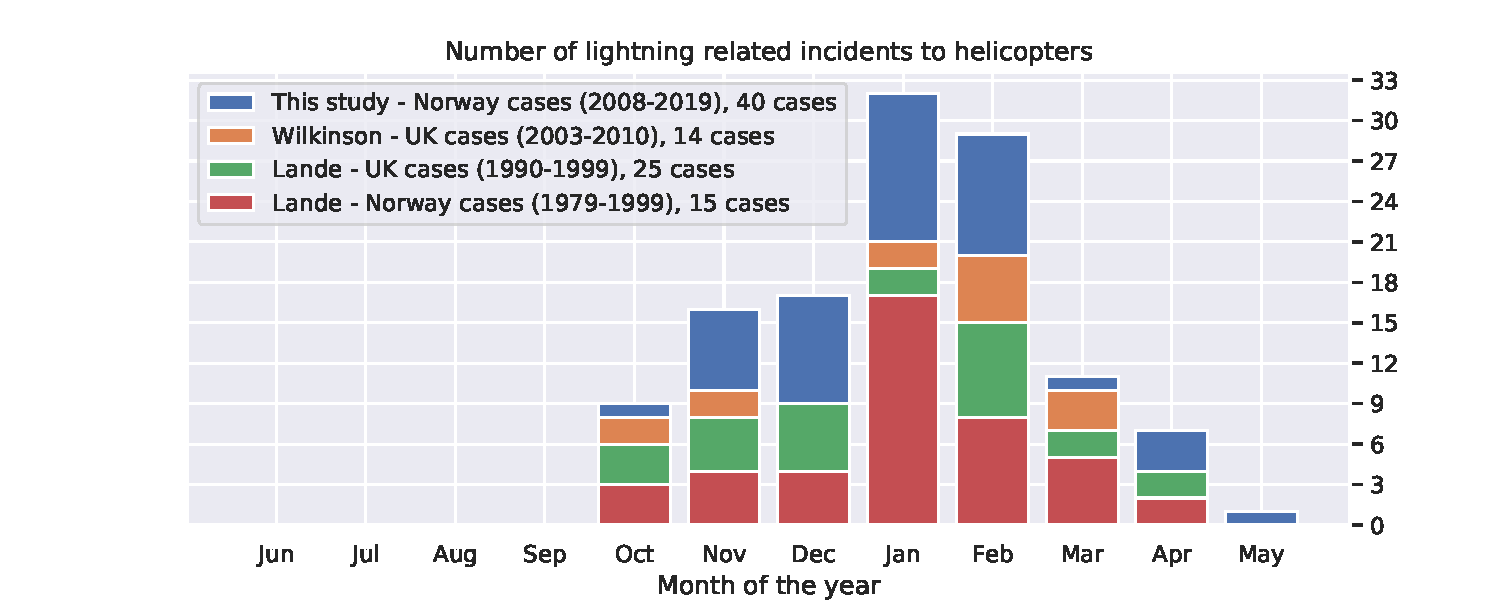
\includegraphics[width=\textwidth]{Figures/yearlydistribution.pdf}
    \label{fig:landewilk}
\end{figure}

The study of \acrshort{htl} has a long history, but had its peak around the turn of the century, due to two helicopter accidents related to lightning (1995 and 2002). This resulted in practical guidelines to helicopter pilots based on data from earlier incidents (\cite{lande}, \cite{hardwick}). Furthermore, \cite{wilkinson} adds numerical simulation and forecasting to this, with the \acrfull{hti}, to provide a more robust and spatially spread warning to be used by helicopter pilots. Since then, there have been improvements in forecasts from numerical weather prediction models due to better physical understanding, better and more observations, and increase in CPU availability. I therefore in this study use the \acrfull{era5} dataset to investigate the atmospheric conditions during helicopter triggered lightning incidents and a similar phenomenon \acrfull{fwtl}. \acrshort{fwtl} is triggered lightning involving planes and rockets, where the wings are fixed. I use a dataset from Avinor with both \acrshort{fwtl} and \acrshort{htl} to identify cases to investigate. I also use the operational \acrfull{meps} to investigate cases that have occurred since November 2016, when \acrshort{meps} began. \acrshort{meps} also provides higher temporal and spatial resolution compared to \acrshort{era5}. Further I utilize the \acrshort{meps}-ensemble members to assess if this can provide improved forecast ability for \acrshort{htl}.

I utilize these methods to improve and strengthen the confidence in the current operational \acrshort{htl} forecast. I also investigate an error found in the operational forecast where the accumulated precipitation, and not the intended hourly precipitation was used in the operational forecast. This have lead to a potential over-estimation of risk related to offshore flights.

These are the research questions I attempt to answer:
\begin{itemize}	
    \item Is Helicopter Triggered Lightning forecasted well?
    \item What atmospheric conditions are present for an \acrshort{fwtl}-event and can \acrshort{fwtl} be used as a proxy for \acrshort{htl}? 
    \item Can the forecast be improved by using an ensemble approach?
\end{itemize}






